\documentclass[a4paper,11pt]{jsarticle}

\renewcommand{\figurename}{Fig.}
\renewcommand{\tablename}{Table }
\usepackage[top=30truemm,bottom=30truemm,left=25truemm,right=25truemm]{geometry}
\usepackage{amsmath,amsfonts}
\usepackage{bm}
\usepackage[dvipdfmx]{graphicx}
\usepackage{booktabs}
\usepackage{array}
\usepackage{multirow}
\usepackage{here}
\usepackage{array}
\usepackage{tabu}
\usepackage{wrapfig}
\usepackage{siunitx}


\begin{document}

\title{たわみ振動によるヤング率の測定}
\author{1522063 手塚裕貴}
\date{実験日 2023 年 6月 13日, 6月 20日}
\maketitle

\begin{abstract}
この実験の目的は、固体の弾性率の測定方法の一種である「振動リード法」を用いて、板状試料と針金状試料
のヤング率と減衰率を測定し、文献値と比較することで、試料物質を特定することである。
概要は以下の通りである。
与えられた板状試料と針金状試料に対して、
密度とヤング率を測定し、文献値と比較して試料の種類の推測を行った。
結果、板状試料は炭素鉄、針金状試料は銅(C1020)であることが得られた。
板状試料については、密度とヤング率のいずれも文献値と近い値が得られたが、針金状資料は長さに歪みが生じやすく、長さを正確に測れていなかったため、ヤング率に大きな誤差が生じた。

\end{abstract}


\section{Introduction}
個体の弾性率を測定する方法は大きく分けると、試料に応力を与えて歪みを測る「静的方法」、試料を振動させて共振周波数を測る「動的方法」、試料の大きさに対して波長が十分に短い弾性波のパルスを試料に当てて波の通過時間を測る「パルス法」の三種類がある。本実験では「動的方法」の一種で、板状、針金状試料の弾性率の測定に有効な「振動リード法」でヤング率と減衰率の測定を行った。
\section{Theoretical background}
\subsection{一端固定、一端自由のたわみ振動のヤング率}
試料板の一端を固定し,もう一端を振動させた場合の共振周波数$f_r$は:
\begin{equation}
  f_r^2 = \frac{a_n^4 k^2 E}{4 \pi^2 l^4 \rho}
\end{equation}
で与えられる。
$a_n$は振動の次数による定数で、基本振動に対して$a_0 = 1.875$、第1、第2次振動に対して$a_1=4.694$、$a_2=7.855$で
ある。
$k^2$は板の断面の形による定数で、厚さ$d$の板の場合$k^2 = d^2/12$である。半径$r$の円棒の場合$k^2 = r^2/4$である。 $E$はヤング率、$l$は試料の長さ、$\rho$は密度である。よって、共振周波数$f_r$を測定し(1)式よりヤング率$E$を求める。
\subsection{Lorentzian関数によるフィッティング}
Fig.1のように周波数-振幅特性には、Lorentzian関数の形が現れる。これは、減衰振動する運動方程式の虚数解が由来する。
Lorentzian関数は次のように表される:
\begin{equation}
  f(x) = \frac{a}{1 + (\frac{x - x_0}{b})^2} + c
\end{equation}
$x = x_0$の時、$f(x)$は最大値を取るので、共振周波数に$x_0$対応する。
各パラメータ$a, b, c$は、測定した各周波数での振幅の測定値に対して、$f(x)$との残差の二乗和が最小になるように決定される。
\begin{figure}[H]
  \center
  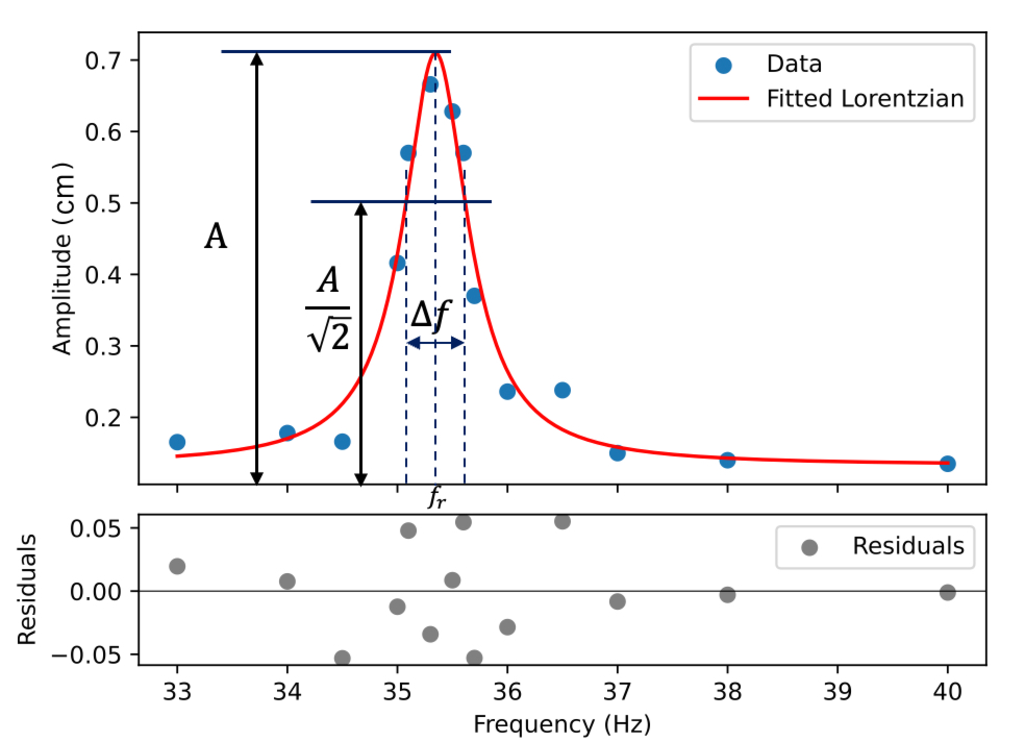
\includegraphics[width=0.6\textwidth]{figs/attenuation_1.pdf}
  \caption{Frequency-Amplitude Characteristics}
\end{figure}
\subsection{減衰率}
減衰率$Q^{-1}$は、エネルギーの損失を定量的に表す量で、振動が一周期するたびにエネルギーがどの程度失われるかを表す値であり、
減衰率$Q^{-1}$は、fig.1に示すように振幅の極大値を$f_r$、極大値の$\frac{1}{\sqrt{2}}$になる両端の周波数の差を$\Delta f$とするとき以下の式で与えられる:
\begin{equation}
  Q^{-1} = \frac{\Delta f}{f_r}
\end{equation}
\section{Experimental procedures}
\subsection*{使用器具}
低周波発振器(型番:FGX-2005)、遊尺顕微鏡、加振器、電気スタンド、ノギス、マイクロ
メーター、電子天秤、板状試料、針金状試料
\subsection{試料の測定方法}
\begin{figure}[H]
  \centering
  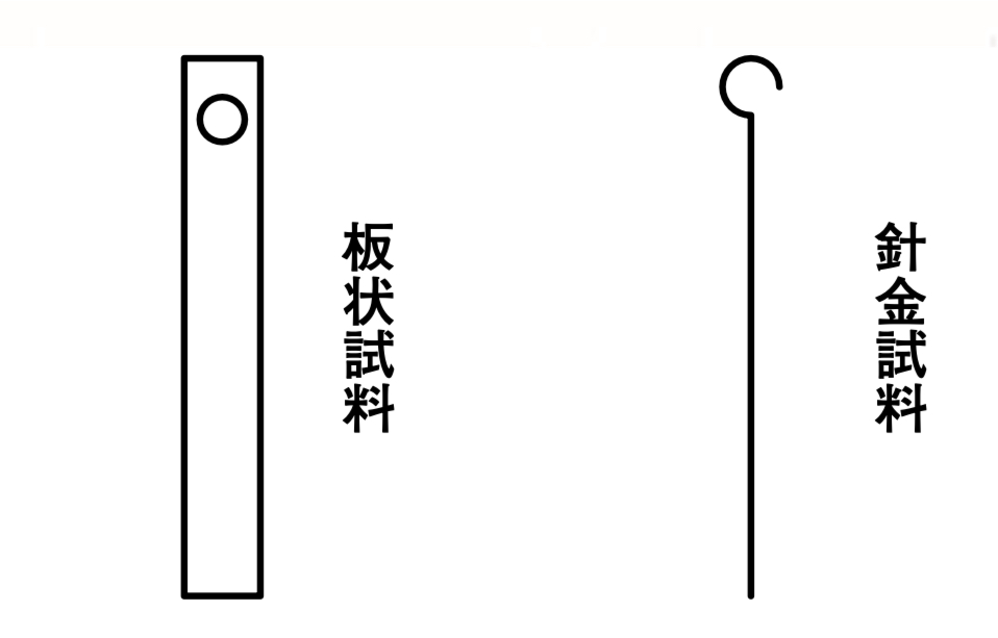
\includegraphics[width=0.5\textwidth]{figs/shape_sample.pdf}
  \caption{Sample Shape}
\end{figure}
実験で扱った試料は、Fig.2のような板状試料と針金状試料である。
ノギス、マイクロメーターを用いて、板状試料の、長さ$l$、幅$w$、厚さ$t$、針金状試料の、長さ$l$、直径$d$を測定した。
また、電子天秤を用いて、質量$m$を測定した。
\subsection{基本振動の共振周波数の測定方法}
\begin{figure}[H]
  \centering
  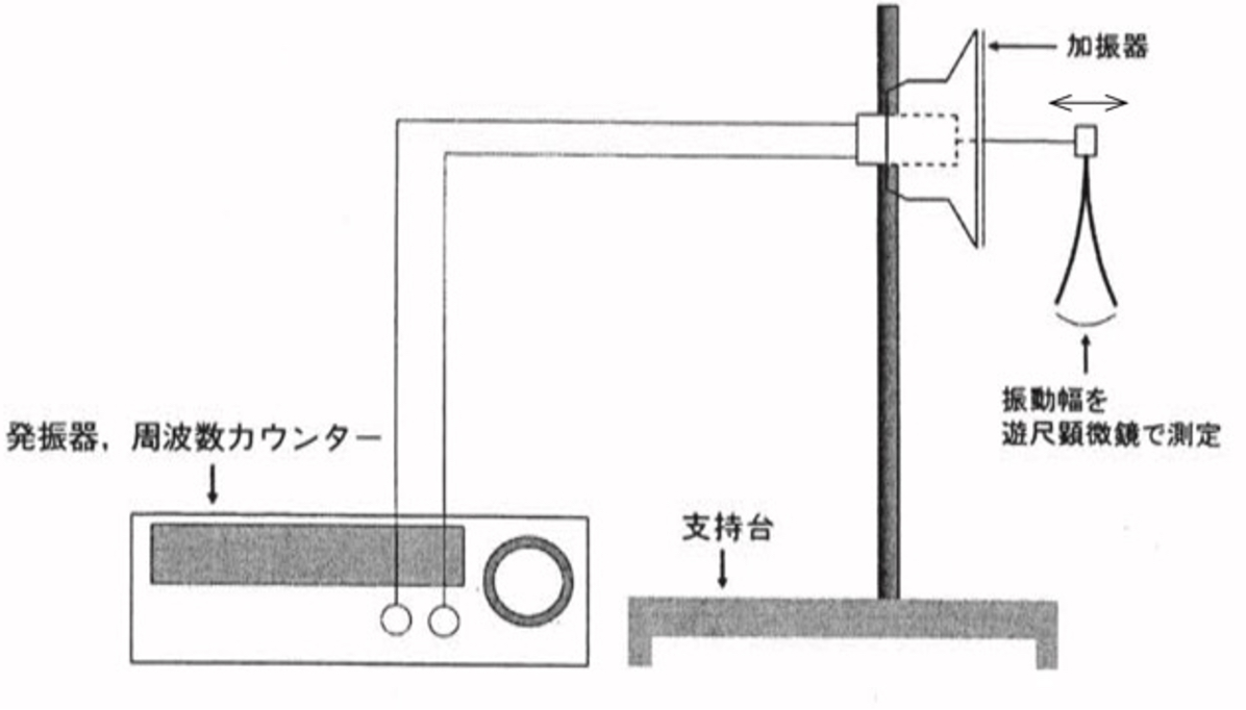
\includegraphics[width=0.5\textwidth]{figs/device_sample.pdf}
  \caption{Schematic diagram of the experimental equipment}
\end{figure}
共振周波数はFig.3のような実験装置を接続して測定した。
左下の発信器を用いることで特定の周波数を発生させ、その振動を加振器を用いて試料に伝える。試料を基本振動近傍で振動させ、その際の振幅を遊尺顕微鏡で観測した。
遊尺顕微鏡には、下に目盛がついており、振動先端の左端と右端の目盛を位置を読み取ることで、差分から振幅を計算した。
遊尺顕微鏡で振幅を測る際は、電気スタンドを用いることで振幅が鮮明に見えるようにした。
すると、振幅-周波数グラフの測定点が得られる。各測定点から、近似曲線を引くことで、共振周波数を求めた。
\clearpage
\section{Results}
\subsection{基本振動の測定結果(板状試料)}
基本振動の共振周波数周辺で、周波数を変化させて板状試料の振幅を測定した。
その結果がFig.4である。
横軸周波数、縦軸振幅であり、青色の点は実測値、赤色の線はLorentzian関数でフィッティングをした結果である。
下の散布図は、データの実測値とモデルによる予測値の差分を表している。
フィッティングには、Pyhtonのlmfitライブラリを用いた。

\begin{figure}[H]
  \centering
  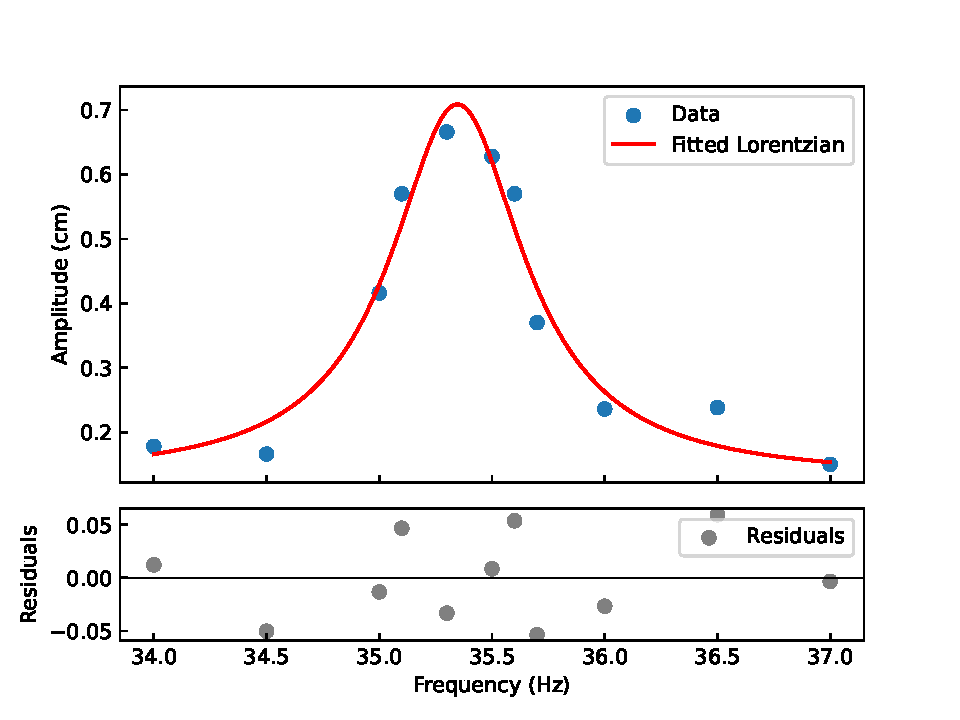
\includegraphics[width=0.7\textwidth]{figs/fitting_Lorentzian.pdf}
  \caption{Relationship between frequency and amplitude(Plate sample)}
\end{figure}
得られたLorentzian関数の式は以下のようになった:
\begin{equation}
  f(x) = \frac{0.6589}{1 + (\frac{x - 35.34}{0.3604})^2} + 0.1269 
\end{equation}
誤差を含めた共振周波数は、$f_r = 35.34 \pm 0.02$[Hz]と求められた。

\subsection{基本振動の測定結果(針金状試料)}
板状試料を同様、針金状試料の基本振動の共振周波数周辺で、周波数を変化させて針金状試料の振幅を測定した。
その結果がFig.5である。
\begin{figure}[H]
  \centering
  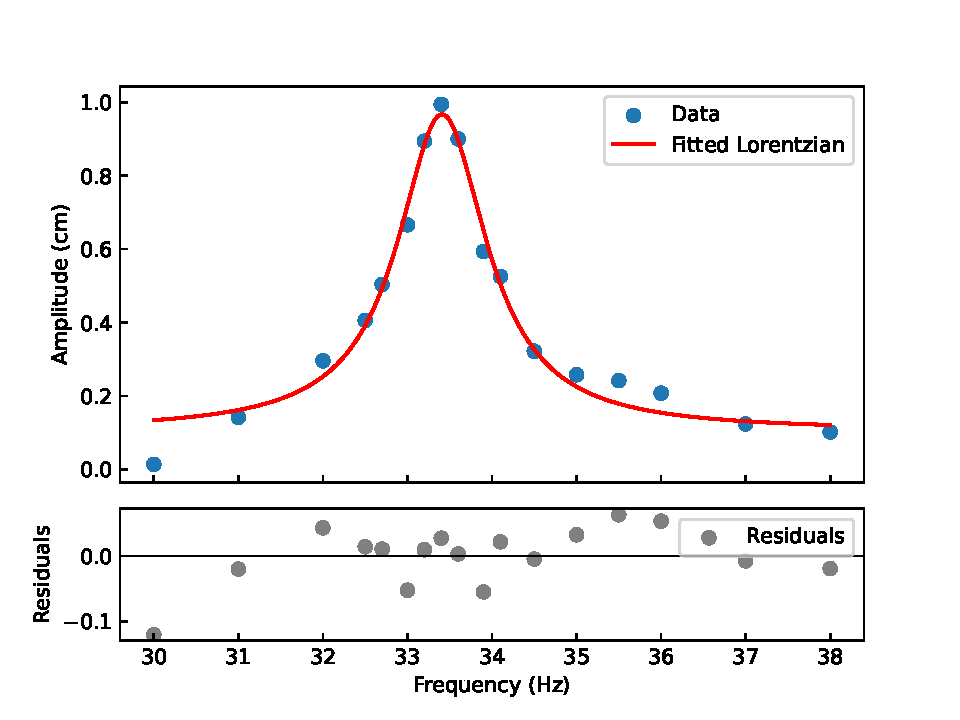
\includegraphics[width=0.7\textwidth]{figs/fitting_Lorentzian2.pdf}
  \caption{Relationship between frequency and amplitude(Wire sample)}
\end{figure}
プロット点が多く、周波数の測定範囲を狭く取ってしまったため、フィッティングが偏っていることがわかる。幸い、共振周波数の値には大きな影響を与えないため、このまま共振周波数を求めた。
得られたLorentzian関数の式は以下のようになった:
\begin{equation}
  f(x) = \frac{1.739}{1 + (\frac{x - 33.40}{0.6423})^2} + 0.1046
\end{equation}
誤差を含めた共振周波数は、$f_r = 33.40 \pm 0.03$[Hz]と求められた。

板状試料、針金状試料の測定結果は以下の表にまとめた。求まった密度はそれぞれ、7.598 [g/cm$^3$]、8.466 [g/cm$^3$]であった。
% Table generated by Excel2LaTeX from sheet '_________'
\begin{table}[H]
  \centering
  \caption{Measurement results for plate samples}
    \begin{tabular}{rrrrr}
    \multicolumn{1}{l}{wisth[mm]} & \multicolumn{1}{l}{length[mm]} & \multicolumn{1}{l}{thickness[mm]} & \multicolumn{1}{l}{Radius of hole [mm]} & \multicolumn{1}{l}{weight[g]} \\
    \midrule
    5.05  & 70    & 0.199 & 1.505 & 0.525 \\
    5     & 70    & 0.2   & 1.50375 &  \\
    5     & 70.05 & 0.199 & 1.505 &  \\
    5     & 70.1  & 0.202 & 1.505 &  \\
    5     & 70    & 0.205 & 1.50375 &  \\
    \end{tabular}%
  \label{tab:addlabel}%
\end{table}%
% Table generated by Excel2LaTeX from sheet '_________'
% Table generated by Excel2LaTeX from sheet '________'
\begin{table}[H]
  \centering
  \caption{Measurement results of wire samples}
    \begin{tabular}{rrr}
    \multicolumn{1}{l}{length[cm]} & \multicolumn{1}{l}{radius[mm]} & \multicolumn{1}{l}{weight[g]} \\
    \midrule
    13.4  & 1.03  & 0.9267 \\
    13.3  & 1.02  &  \\
    13.4  & 1.03  &  \\
    13.25 & 1.02  &  \\
    13.1  & 1.02  &  \\
    \end{tabular}%
  \label{tab:addlabel}%
\end{table}%

振幅-周波数の測定値は以下の表にまとめた。
% Table generated by Excel2LaTeX from sheet '________'
\begin{table}[H]
  \begin{minipage}{0.5\hsize}
    \centering
    \caption{Measurement results for plate samples}
      \begin{tabular}{rr}
      \multicolumn{1}{l}{Frequency [Hz]} & \multicolumn{1}{l}{amplitude [cm]} \\
      \midrule
      35.5  & 0.628 \\
      36    & 0.236 \\
      36.5  & 0.238 \\
      35.3  & 0.666 \\
      35.7  & 0.37 \\
      37    & 0.15 \\
      35    & 0.416 \\
      34.5  & 0.166 \\
      35.6  & 0.57 \\
      35.1  & 0.57 \\
      34    & 0.178 \\
      33    & 0.1653 \\
      &  \\
      &  \\
      &  \\
      &  \\
      &  \\

      \end{tabular}%
  \label{tab:addlabel}%
  \end{minipage}
  \begin{minipage}{0.5\hsize}
    \centering
    \caption{Measurement results of wire samples}
    \begin{tabular}{rr}
    \multicolumn{1}{l}{Frequency [Hz]} & \multicolumn{1}{l}{amplitude [cm]} \\
    \midrule
    30    & 0.014 \\
    31    & 0.142 \\
    32    & 0.296 \\
    32.5  & 0.406 \\
    32.7  & 0.504 \\
    33    & 0.666 \\
    33.2  & 0.894 \\
    33.4  & 0.994 \\
    33.6  & 0.9 \\
    33.9  & 0.594 \\
    34.1  & 0.526 \\
    34.5  & 0.322 \\
    35    & 0.258 \\
    35.5  & 0.242 \\
    36    & 0.208 \\
    37    & 0.124 \\
    38    & 0.102 \\
    \end{tabular}%
  \end{minipage} 
\end{table}%

\clearpage

\section{Discussion}
\subsection{ヤング率の導出と文献値との比較}
(1)式より、ヤング率を求めた。

板状試料のヤング率は$ 2.16 \times 10^{11}$[kg/m$\cdot \text{s}^2$]、
針金状試料のヤング率は$ 7.36 \times 10^{10}$[kg/m$\cdot \text{s}^2$]
となった。

密度とヤング率を文献値と比較して求めると、
板状試料は密度、ヤング率ともに、炭素鉄(s45c)(密度:$7.59$[g/$\text{cm}^3$]、ヤング率:$2.16\times 10^{11}$[kg/m$\cdot \text{s}^2$])が最も近い値となった。一方、針金状試料は密度が最も近い値は銅(C1020)であったが、ヤング率は$1.29\times 10^{11}$[kg/m$\cdot \text{s}^2$]と大きくずれていた。
針金状試料のヤング率は文献値と大きくずれたが、密度からして銅になると推測し、式(1)から誤差を生み出したのは長さlの影響が大きいと考え、($l$の4乗に比例)lを逆算して計算した結果、$l = 12.80$ cmであった。
試料の長さを正しく測れていなかった可能性が高い。

\subsection{振幅-周波数特性にLorentzian関数が現れる物理的背景}
角振動数$\omega$の外力を受けながら減衰振動する質量$m$の運動方程式は以下で与えられる:
\begin{equation}
  m\Bigl( \frac{d^2}{dt^2} x(t) + \gamma \frac{d}{dt}x(t) + \omega_0^2 x(t)\Bigr) = f_0 \exp(i\omega t)
\end{equation}
共振周波数近傍に注目し、$\omega \approx \omega_0$とすると、虚数解:
\begin{equation}
  x = -\frac{f_0 \gamma / 4\omega_0 m}{(\omega_0 - \omega)^2 + (\gamma /2)^2}
\end{equation}
から、Lorentzian関数が現れる。また、運動方程式の第二項から$\gamma$は減衰係数であることがわかる。
\subsection{減衰率の導出}
\subsection{(1)式の導出}
一端固定、一端自由のたわみ振動を考える。
この時の振動は、物体が弾性波を伝播させることによって生じる。
弾性波の速度$v$は、物体のヤング率$E$と密度$\rho$によって決まり、次のように表される:
\begin{equation}
  v = \sqrt{\frac{E}{\rho}}
\end{equation}
一方、弾性波の周波数$f$は、波の速度$v$と波長$\lambda$によって決まり、次のように表される:
\begin{equation}
  f = \frac{v}{\lambda}
\end{equation}
片持ち梁の最低の共振周波数(基本振動)は、波長が梁の長さの2倍(つまり $\lambda=2l$)
の時に実現される。
したがって、基本振動数$f_r$は次のように表される:
\begin{equation}
  f_r = \frac{v}{2l} = \frac{v}{2l}\sqrt{\frac{E}{\rho}}
\end{equation}
これを二乗すると次の式が得られる:
\begin{equation}
  f_r^2 = \frac{1}{4l^2}\frac{E}{\rho}
\end{equation}
振動の次数による定数、試料の断面に依る係数を加えてやると、最終的には:
\begin{equation}
  f_r^2 = \frac{A}{4\pi l^4}\frac{E}{\rho} 
\end{equation}
したがって、$E$について解くと
\begin{equation}
  E = \frac{4\pi l^4 \rho}{A}f_r^2
\end{equation}
この式から、ヤング率$E$を求めるには、試料の長さ$l$、密度$\rho$、共振周波数$f_r$を求めれば良いことになる。
\section{Conclusion}
「振動リード法」を用いて、板状試料と針金状試料
のヤング率と減衰率を測定し、文献値と比較することで、試料物質を特定した。
その結果、密度とヤング率の測定から、板状試料は炭素鉄、針金状試料は銅(C1020)であることが得られた。

\begin{thebibliography}{文献数}
\bibitem{ID} 参考文献の名前・著者1
\bibitem{ID2} 参考文献の名前・著者2
\bibitem{ID3} 参考文献の名前・著者3
\end{thebibliography}

\end{document}